\newpage
\subsection{Multivariate Analysis}

\quad The Multivariate Analysis is similiar to the Univariate Analysis, the diference is that in this one we will use more than a set of data, in this project we will use the precipitation and the maximum temperature to assiste in the prediction of sales for each of the drinks.\\


We try multiple neural networks architectures, with LSTM, to find which is the most efficient for our project:

\begin{figure}[H]
    \centering
    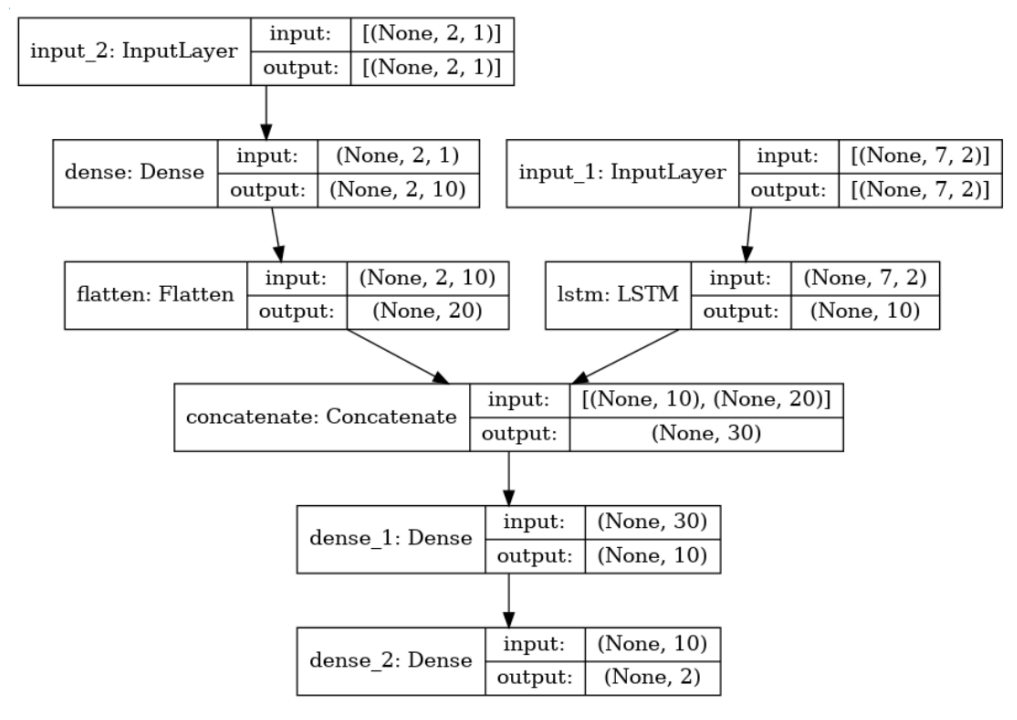
\includegraphics[width=0.8\textwidth]{assets/mult4.png}
    \caption{Neural Network architecture 1}
    \label{fig:neural_network}
    \end{figure}

    \begin{figure}[H]
        \centering
        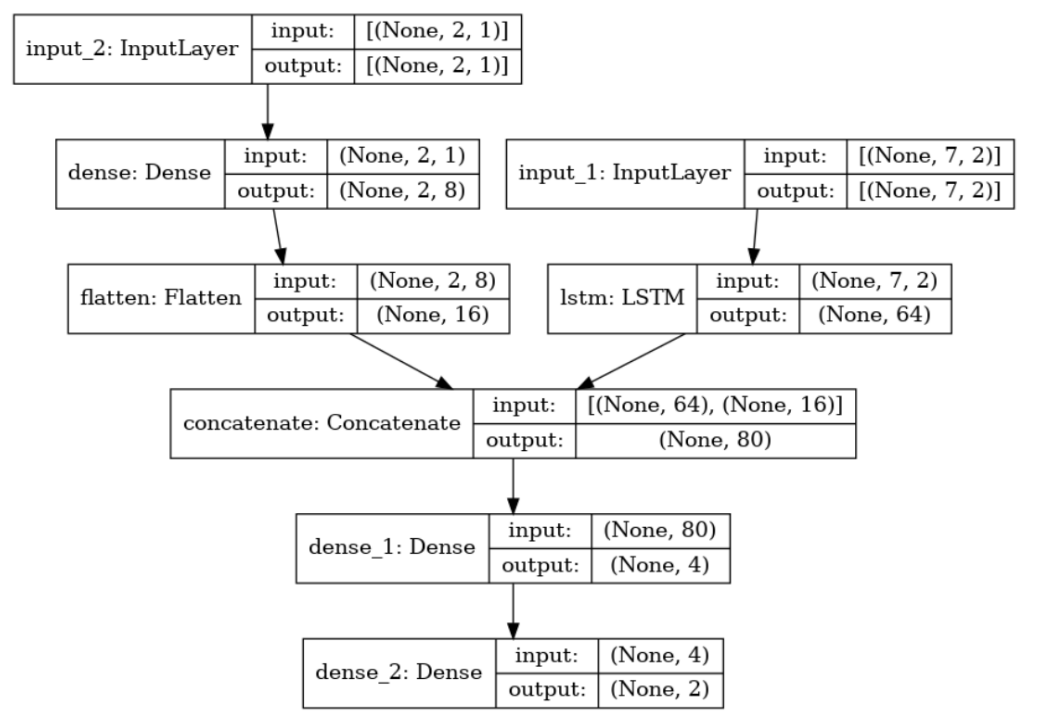
\includegraphics[width=0.8\textwidth]{assets/mult5.png}
        \caption{Neural Network architecture 2}
        \label{fig:neural_network}
        \end{figure}

        \begin{figure}[H]
            \centering
            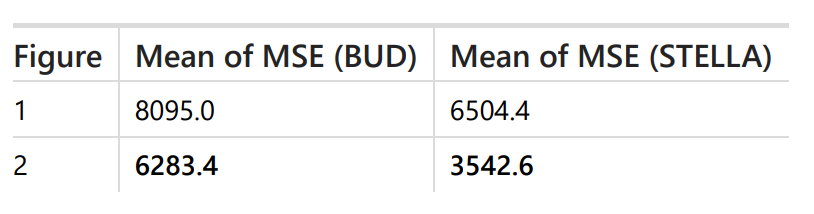
\includegraphics[width=0.8\textwidth]{assets/mult6.png}
            \caption{Neural Network Average MSE}
            \label{fig:neural_network}
            \end{figure}

As we can see from the image above, we conclude that the best neural network architectures is the second one.\\


We tried another approach with the following architecture:

\begin{figure}[H]
    \centering
    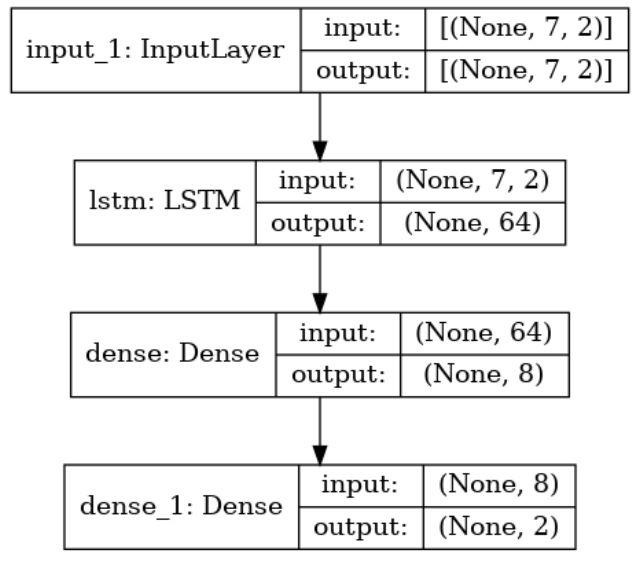
\includegraphics[width=0.8\textwidth]{assets/mult10.jpeg}
    \caption{Alternative Neural Network}
    \label{fig:neural_network}
    \end{figure}


    \begin{figure}[H]
        \centering
        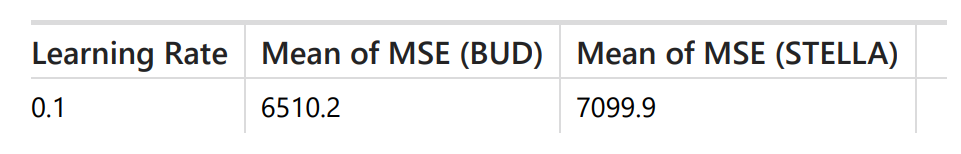
\includegraphics[width=0.8\textwidth]{assets/mult8.png}
        \caption{Alternative Neural Network Average MSE}
        \label{fig:neural_network}
        \end{figure}
    

As we can see the approach before have better results than the alternative.\\


For the prediction we will use a split of Growing Window to predict the last 20 weeks of sales, for each drink, with a step of 7. The next image represents the results of the average error MSE of the 20 weeks prediction:\\


\begin{figure}[H]
    \centering
    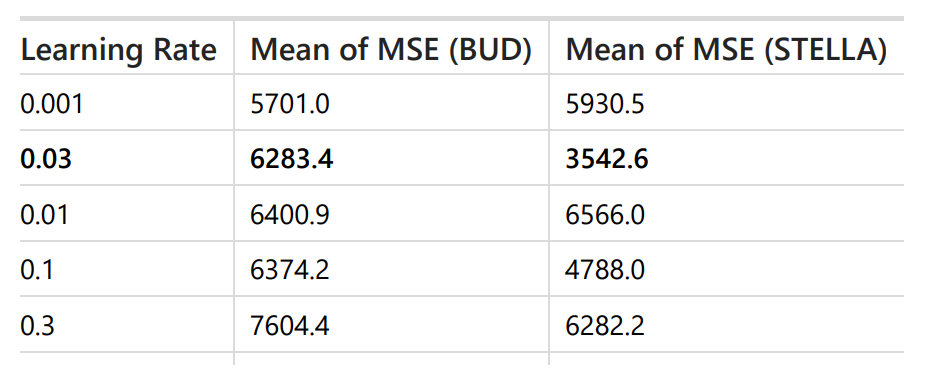
\includegraphics[width=0.4\textwidth]{assets/mult7.png}
    \caption{Average of MSE Error for STELLA and BUD}
    \label{fig:notas}
    \end{figure}

For demonstration purposes here are the graphics of each of the predictions made for the BUD and STELLA:\\

\begin{figure}[H]
    \centering
    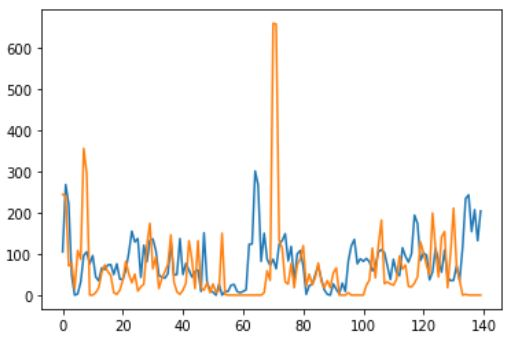
\includegraphics[width=0.6\textwidth]{assets/multt-stella.jpeg}
    \caption{STELLA - Multivariate Analysis Results}
    \label{fig:notas}
    \end{figure}

\begin{figure}[H]
    \centering
    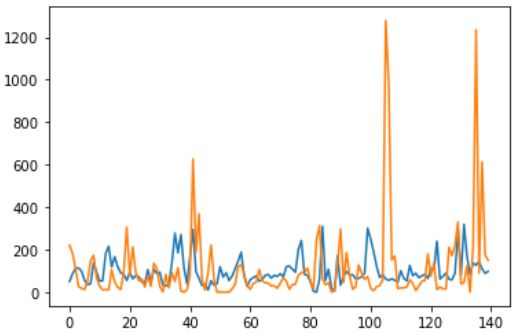
\includegraphics[width=0.6\textwidth]{assets/multt-bud.jpeg}
    \caption{BUD - Multivariate Analysis Results}
    \label{fig:notas}
    \end{figure}



    For last step we use the Weekly Naive as the standard metric to compare wwith the best result:\\

    \begin{figure}[H]
        \centering
        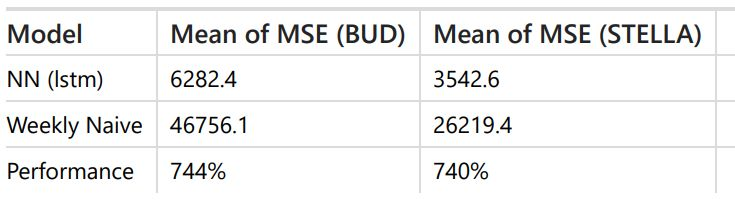
\includegraphics[width=0.6\textwidth]{assets/mult11.jpeg}
        \caption{Weekly Naive Results}
        \label{fig:notas}
        \end{figure}    

As we can see the STELLA results are 7.4 times better and the BUD results are 7.44 times better.




